\section{PTracking Algorithm}

\begin{frame}
	\frametitle{PTracking algorithm}
	
	\vspace{0.6cm}
	
	\textbf{Global recursive update}
	
	\vspace{-0.4cm}
	
	\begin{eqnarray*}
	p(x_t|z_{1:t-1}^\mathcal{A}) &=& \int p(x_t|x_{t-1}) p(x_{t-1}|z_{1:t-1}^\mathcal{A})dx_{t-1}, \\
	p(x_t|z_{1:t}^\mathcal{A}) &=& \frac{p(z_t^\mathcal{A}|x_t) p(x_t|z_{1:t-1}^\mathcal{A})}{\int p(z_t^\mathcal{A}|x_t)p(x_t|z_{1:t-1}^\mathcal{A})dx_t}.
	\end{eqnarray*}
	
	\textbf{GMM parameters}
	
	\vspace{-0.1cm}
	
	\begin{equation*}
		\mu_t^c = \frac{\sum_{i=1}^N x_t^{(i)}\lambda_t(c|x_t^{(i)})}{\sum_{i=1}^N \lambda_t(c|x_t^{(i)})},\;\;\;\;\;\;\;
		\sigma_t^c = \frac{\sum_{i=1}^N (x_t^{(i)} - \mu_t^c)^2\lambda_t(c|x_t^{(i)}) }{\sum_{i=1}^N \lambda_t(c|x_t^{(i)}) }.
	\end{equation*}
	
	\emph{where}
	
	\vspace{-0.5cm}
	
	\begin{equation*}
		\lambda_t(c|x_t^{(i)}) = \frac{\mathcal{N}(x_t^{(i)},\mu_t^c,\sigma_t^c)\lambda_t^c} {\sum_{m=1}^{\mathcal{C}}\mathcal{N}(x_t^{(i)},\mu_t^m,\sigma_t^m)\lambda_t^m},\;\;\;\;\;\;\;
		\lambda_t^c = \frac{1}{N} \sum_{i=1}^N \lambda_t(c|x_t^{(i)}),
	\end{equation*}
\end{frame}

\begin{frame}
	\frametitle{PTracking algorithm}
	
	\Large
	
	\begin{itemize}
		\item \textbf{Input:} a set of positions of the objects provided by a multi-object detection system
		
		\vspace{0.4cm}
		
		\item \textbf{Output:} the estimated trajectories of the moving objects over time
	\end{itemize}
\end{frame}

\begin{frame}
	\frametitle{PTracking algorithm}
	
	\only<1->
	{
		\large
		Each agent runs a two-tiered distributed algorithm
	}
	
	\begin{columns}
		\column{0.4\textwidth}
		\centering
		
		\only<1->
		{
			\vspace{0.7cm}
		}
		
		\only<1->
		{
			\begin{tikzpicture}
				\node at (0,0) [draw=black,ultra thick,inner sep=0pt]  {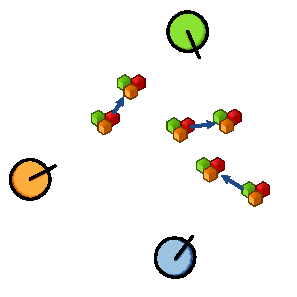
\includegraphics[scale=0.75]{Figures/Mamot}};
			\end{tikzpicture}
		}
		
		\column{0.2\textwidth}
		\centering
		
		\only<2->
		{
			\begin{tikzpicture}
				\node at (0,0) [draw=white,ultra thick,inner sep=0pt]  {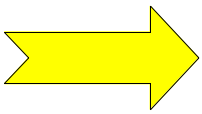
\includegraphics[scale=0.3]{Figures/ArrowRight.png}};
			\end{tikzpicture}
		}
		
		\column{0.4\textwidth}
		\centering
		
		\only<2>
		{
			\begin{tikzpicture}
				\node at (0,0) [draw=black,ultra thick,inner sep=0pt]  {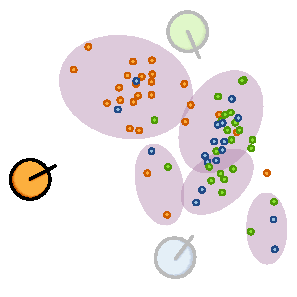
\includegraphics[scale=0.75]{Figures/Mamot2}};
			\end{tikzpicture}
		}
		
		\only<2>
		{
			\vspace{-0.7cm}
		}
		
		\only<3>
		{
			\begin{tikzpicture}
				\node at (0,0) [draw=black,ultra thick,inner sep=0pt]  {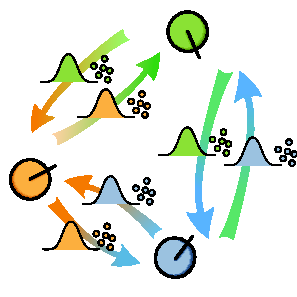
\includegraphics[scale=0.75]{Figures/Mamot3}};
			\end{tikzpicture}
		}
		
		\only<3>
		{
			\vspace{-0.7cm}
		}
		
		\only<4>
		{
			\begin{tikzpicture}
				\node at (0,0) [draw=black,ultra thick,inner sep=0pt]  {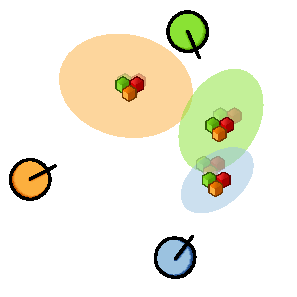
\includegraphics[scale=0.75]{Figures/Mamot4}};
			\end{tikzpicture}
		}
		
		\only<4>
		{
			\vspace{-0.7cm}
		}
	\end{columns}
\end{frame}

\begin{frame}
	\frametitle{Application fields}
	
	\vspace{0.24cm}
	
	\begin{itemize}
		\item Multi-Robot, Single-Object
	\end{itemize}
	
	\vspace{-0.45cm}
	
	\begin{columns}[t]
		\only<1->
		{
			\column{0.75\textwidth}
			
			\begin{block}{Soccer robots}
				used to solve the localization field symmetry problem
			\end{block}
			
			\column{0.2\textwidth}
		}
	\end{columns}
	
	\centering
	\vspace{0.3cm}
	
	\begin{tikzpicture}
				\node at (0,0) [draw=black,ultra thick,inner sep=0pt]  {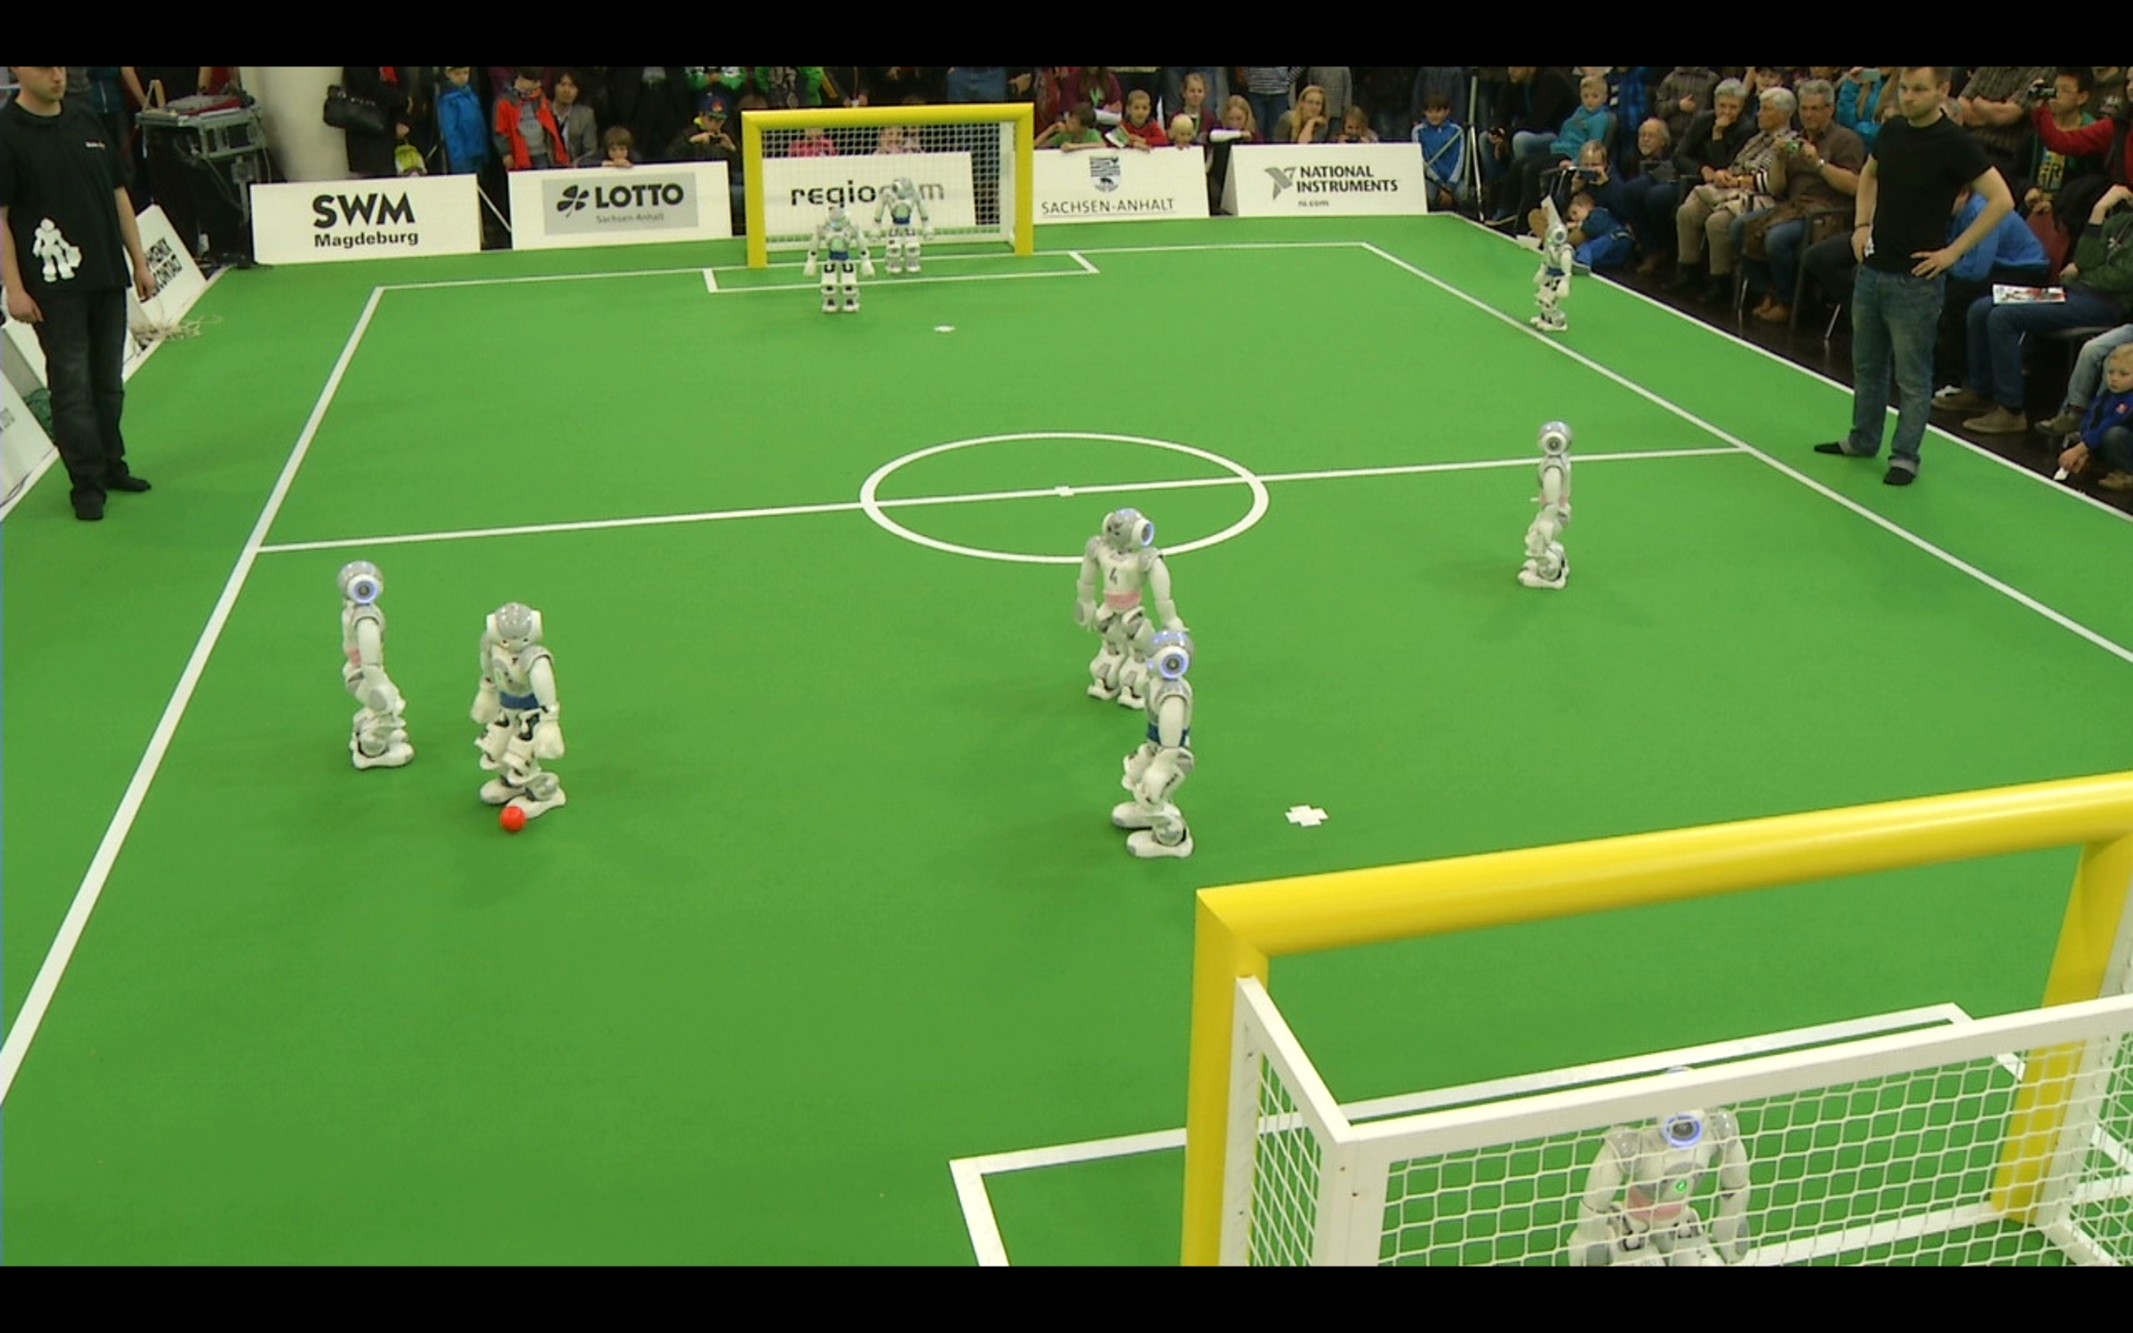
\includegraphics[scale=0.19]{Figures/Naos}};
	\end{tikzpicture}
	
\end{frame}

\begin{frame}
	\frametitle{Application fields}
	
	\vspace{0.455cm}
	
	\begin{itemize}
		\item Multi-Robot, Multi-Object
	\end{itemize}
	
	\vspace{-0.455cm}
	
	\begin{columns}[t]
		\only<1->
		{
			\column{0.35\textwidth}
			\centering
			
			\begin{block}{Prey-Predator game}
				Player/Stage
			\end{block}
			
			\column{0.6\textwidth}
			\centering
			
			\vspace{0.1cm}
			
			\begin{tikzpicture}[map/.style={draw=black,ultra thick,inner sep=0pt}]
				\node at (-3.9,0.8) [map] {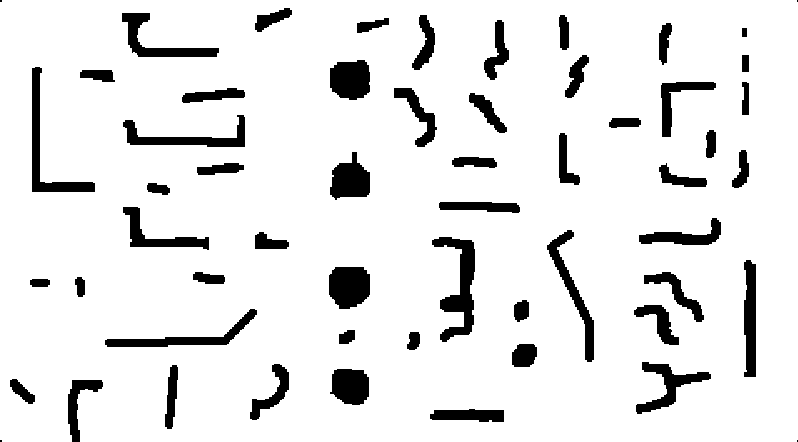
\includegraphics[height=1.1cm]{Maps/Edmonton}};
				\node at (-4.3,1.3) [map] {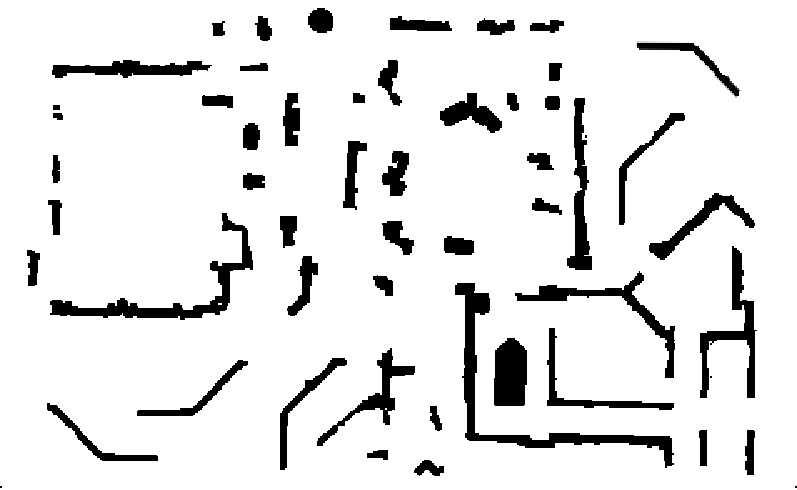
\includegraphics[height=1.1cm]{Maps/Longwood}};
				\node at (-3.0,1.0) [map] {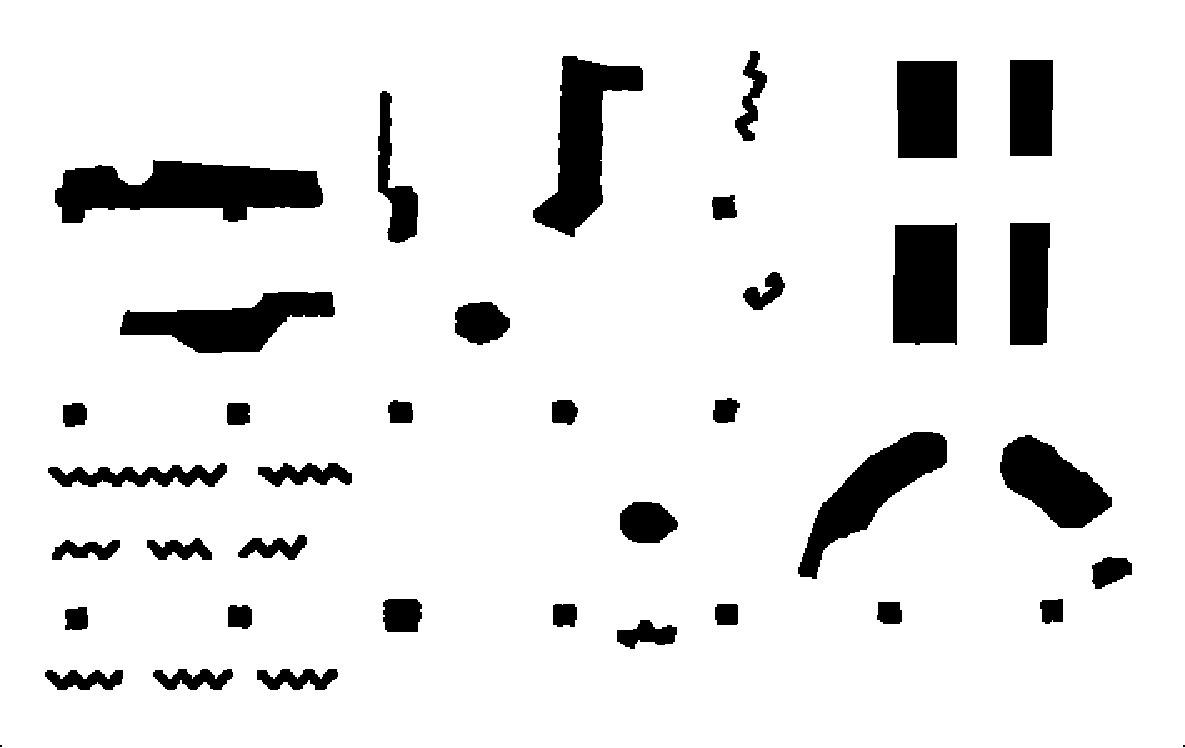
\includegraphics[height=1.1cm]{Maps/Mexico}};
				\node at (-2.8,1.5) [map,draw=red!70!black] {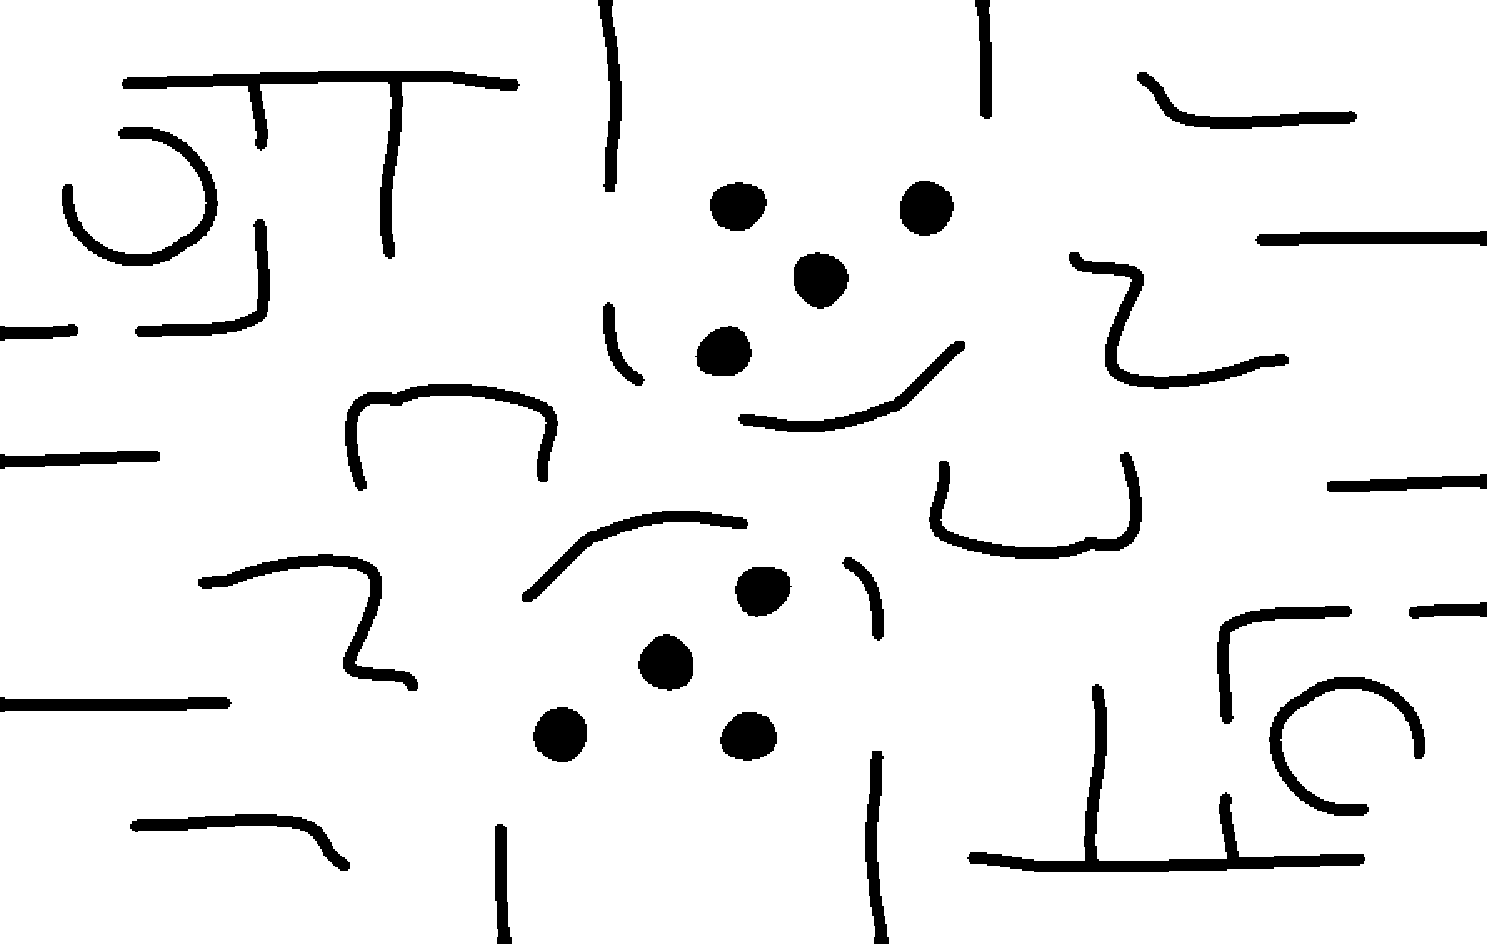
\includegraphics[height=1.25cm]{Maps/Lasermaze}};
			\end{tikzpicture}
		}
	\end{columns}
	
	\vspace{-0.75cm}
	
	\begin{columns}[t]
		\only<1->
		{
			\column{0.55\textwidth}
			\centering
			
			\vspace{0.55cm}
			
			\begin{block}{PETS 2009 dataset}
				Tracking of individuals within a crowd
			\end{block}
			
			\column{0.4\textwidth}
		}
	\end{columns}
	
	\begin{center}
		\begin{tikzpicture}
			\node at (0,0) [draw=black,ultra thick,inner sep=0pt]  {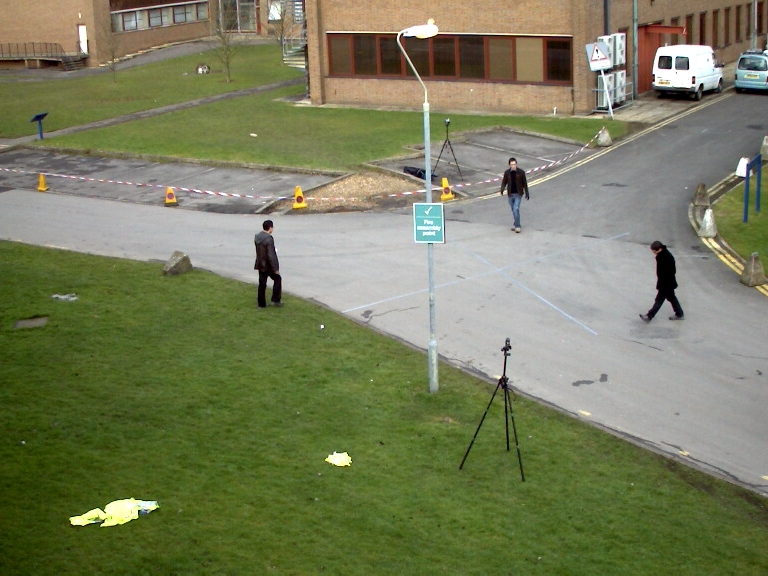
\includegraphics[scale=0.14]{Figures/Pets2009-1.jpg}};
			\node at (4,0) [draw=black,ultra thick,inner sep=0pt]  {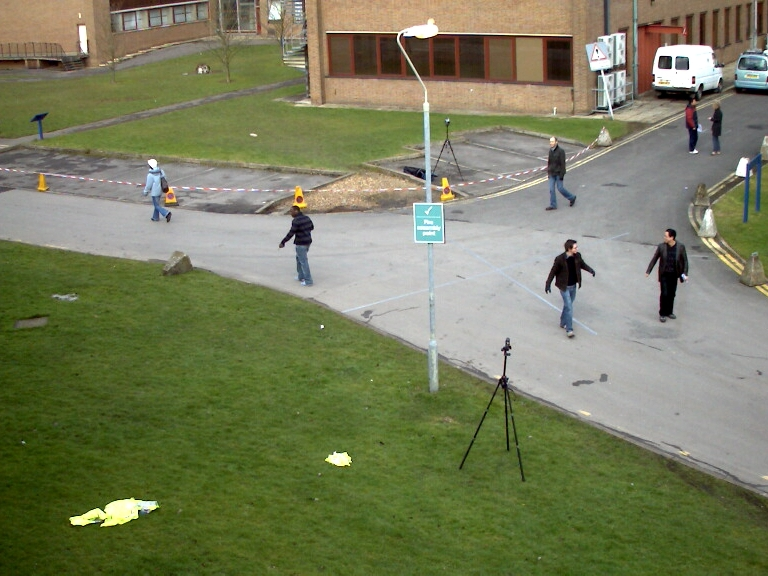
\includegraphics[scale=0.14]{Figures/Pets2009-2.jpg}};
			\node at (8,0) [draw=black,ultra thick,inner sep=0pt]  {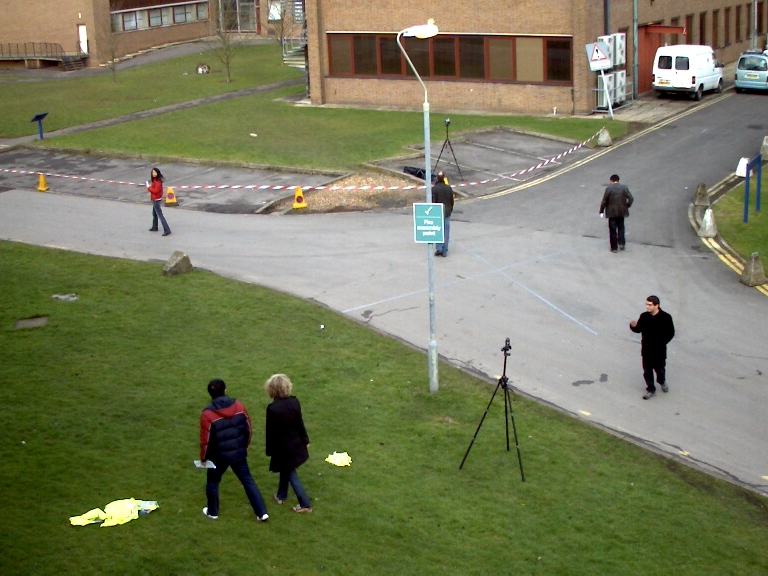
\includegraphics[scale=0.14]{Figures/Pets2009-3.jpg}};
		\end{tikzpicture}
	\end{center}
\end{frame}

\begin{frame}
	\frametitle{A learning approach to Multi-Object Detection and Tracking}
	
	\vspace{-2.5cm}
	
	\only<1->
	{
		\begin{block}{Goal}
			Creating a system that \textbf{can track} objects in an environment using sensors and that is \textbf{able to learn} the behaviours of the tracked objects by applying learning techniques
		\end{block}
	}
	
	\only<2->
	{
		\begin{itemize}
			\item \large\textcolor{red}{Unexplored} open field
		\end{itemize}
	}
	
	\only<2>
	{
		\vspace{-1cm}
	}
	
	\only<3>
	{
		\begin{itemize}
			\item \large\textcolor{red}{Challenges}
			
			\begin{itemize}
				\item \large\textcolor{red}{real-time} object motion detection
				\item objects' \large\textcolor{red}{behavior} recognition
			\end{itemize}
		\end{itemize}
	}
	
	\only<3>
	{
		\vspace{-3.07cm}
	}
\end{frame}

\begin{frame}
	\frametitle{Non-adaptive tracking}
	\framesubtitle{Current state of the art}
	
	\vspace{-3.0cm}
	
	\begin{columns}[t]
		\column{0.7\textwidth}
		
		\only<1->
		{
			\vspace{0.22cm}
		}
		
		\only<1->
		{
			\begin{itemize}
				\item Car park monitoring
				\vspace{0.1cm}
				\newline
				\tiny[\emph{Hampapur et al, ``Smart video surveillance: exploring the concept of multiscale spatiotemporal tracking'', 2005}]
			\end{itemize} 
		}
		
		\only<2->
		{
			\vspace{0.41cm}
		}
		
		\only<2->
		{
			\begin{itemize}
				\item Small objects tracking in aerial video sequences
				\vspace{-0.14cm}
				\newline
				\tiny[\emph{Pless et al, ``Detecting independent motion: the statistics of temporal continuity'', 2000}]
			\end{itemize}
			
			\vspace{0.13cm}
			
			\begin{itemize}
				\item Surveillance system specialized in people tracking
				\vspace{0.1cm}
				\newline
				\tiny[\emph{Haritaoglu et al, ``$ W_4 $: real-time surveillance of people and their activities'', 2000}]
			\end{itemize}
		}
		
		\only<2>
		{
			\vspace{-3.18cm}
		}
		
		\column{0.3\textwidth}
		
		\only<1->
		{
			\begin{tikzpicture}
				\node at (0,0) [draw=black,ultra thick,inner sep=0pt]  {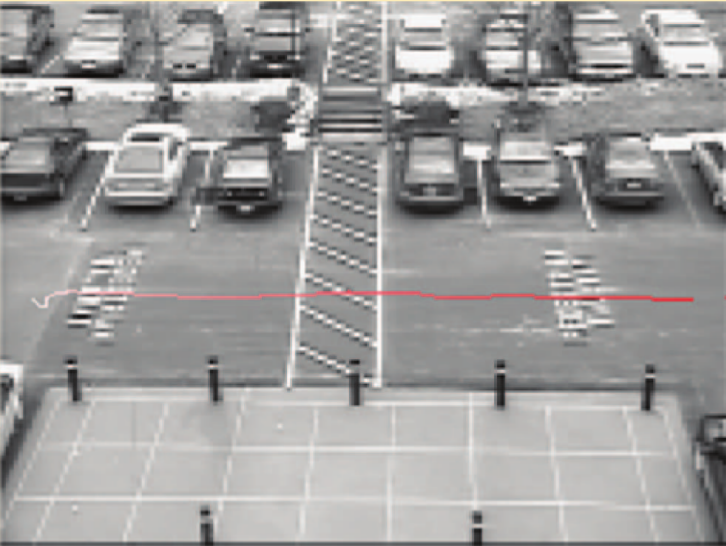
\includegraphics[width=2.3cm]{Figures/CarsPark.png}};
			\end{tikzpicture}
		}
		
		\only<2->
		{
			\begin{tikzpicture}
				\node at (0,0) [draw=black,ultra thick,inner sep=0pt]  {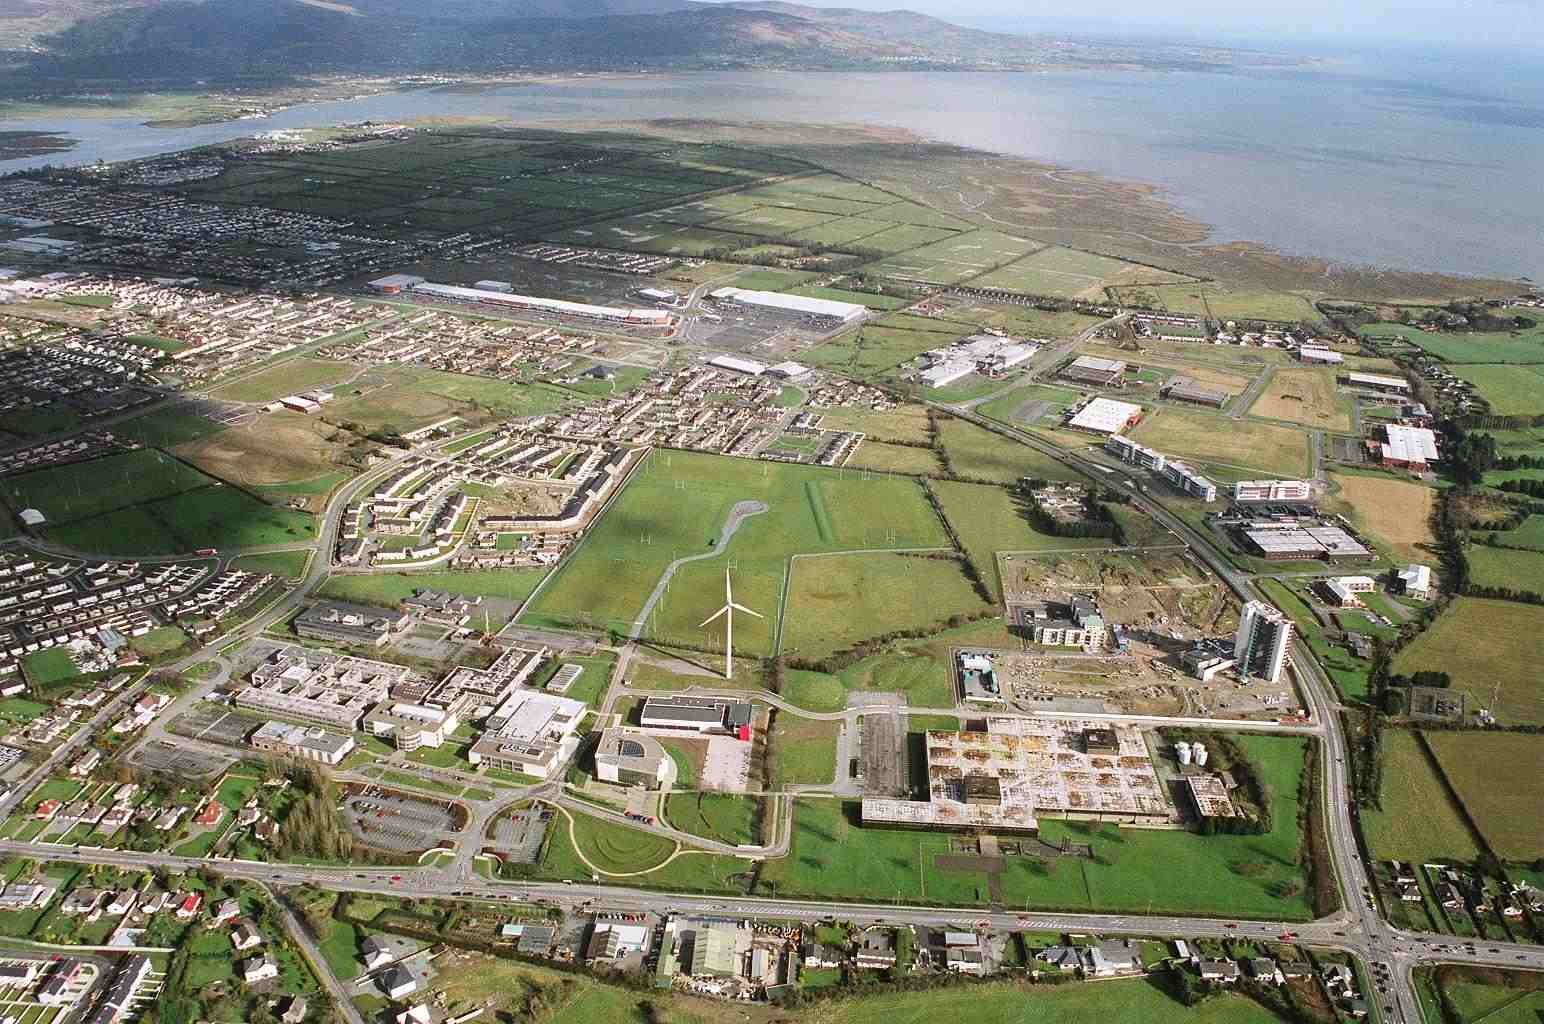
\includegraphics[width=2.3cm]{Figures/Aerial.jpg}};
			\end{tikzpicture}
			
			\begin{tikzpicture}
				\node at (0,0) [draw=black,ultra thick,inner sep=0pt]  {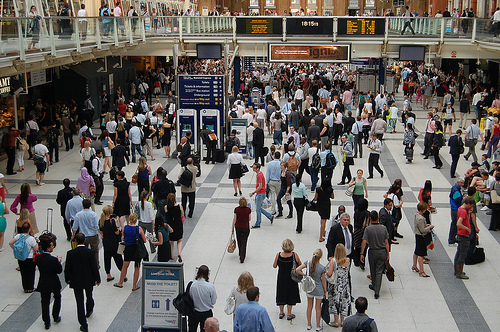
\includegraphics[width=2.3cm]{Figures/FollowingPeople.jpg}};
			\end{tikzpicture}
		}
		
		\only<2>
		{
			\vspace{-5.0cm}
		}
	\end{columns}
\end{frame}

\begin{frame}
	\frametitle{Adaptive tracking}
	
	\only<1>
	{
		\vspace{0.13cm}
	}
	
	\only<1->
	{
		\begin{itemize}
			\item Good results but \textbf{non-adaptive} tracking...
		\end{itemize}
		
		\vspace{-0.5cm}
		
		\begin{tabbing}
			\hspace*{1.0cm}
			
			$ \leadsto $ \textcolor{red}{weak} to environment's changes
		\end{tabbing}
	}
	
	\only<1>
	{
		\vspace{4.05cm}
	}
	
	\only<2->
	{
		\centering
		
		\vspace{-0.2cm}
		
		\begin{tikzpicture}
			\node at (0,0) [draw=white,ultra thick,inner sep=0pt]  {
\includegraphics[scale=0.2]{Figures/ArrowDown.png}};
		\end{tikzpicture}
		
		\textcolor{red}{\textbf{Adaptive tracking}}
		
		\vspace{0.2cm}
		
		\begin{itemize}
			\item \textbf{Small} literature
		\end{itemize}
		
		\vspace{-0.5cm}
		
		\begin{tabbing}
			\hspace*{1.0cm}
			
			$ \leadsto $ \scriptsize[\emph{Stauffer et al, ``Learning patterns of activity using real-time tracking'', 2000}]
		\end{tabbing}
	}
\end{frame}

\begin{frame}
	\frametitle{A learning approach to Multi-Object Detection and Tracking}
	
	\only<1->
	{
		\vspace{-2.4cm}
	}
	
	\only<1->
	{
		An object tracking system \textbf{cannot} be used alone
		
		\begin{itemize}
			\item \emph{system setup}
			
			\item \emph{continuous maintenance after deployment}
		\end{itemize}
	}
	
	\only<2->
	{
		\centering
		
		\begin{tikzpicture}
			\node at (0,0) [draw=white,ultra thick,inner sep=0pt]  {
\includegraphics[scale=0.2]{Figures/ArrowDown.png}};
		\end{tikzpicture}
		
		\vspace{-0.4cm}
		
		\begin{center}
			\textcolor{red}{\textbf{adaptive smart tracking system}}
		\end{center}
		
		$ \leadsto $ the \textcolor{red}{better} is the experience, the \textcolor{red}{better} are the performance over time
	}
	
	\only<2>
	{
		\vspace{-2.99cm}
	}
\end{frame}
